

% !TeX spellcheck = en_US 
\documentclass[12pt,english]{report}
\usepackage{tesi}
% CORSO DI LAUREA:
\def\myCDL{Master in\\Computer Science}

% TITOLO REPORT:
\def\myTitle{Statistical methods for machine learning  \\
\large{Final report on neural networks for the binary classification}}

% AUTORE:
\def\myName{Samuele Simone}
\def\myMat{Matr. Nr. 11910A}

\def\myRefereeA{Prof. Nicolò Cesa-Bianchi}

% ANNO ACCADEMICO
\def\myYY{2022-2023}

% Il seguente comando introduce un elenco delle figure dopo l'indice (facoltativo)
%\figurespagetrue

% Il seguente comando introduce un elenco delle tabelle dopo l'indice (facoltativo)
%\tablespagetrue


% Package di formato
\usepackage[a4paper]{geometry}		% Formato del foglio
\usepackage[english]{babel}			% Supporto per l'italiano
\usepackage[utf8]{inputenc}			% Supporto per UTF-8
\usepackage[a-1b]{pdfx}			% File conforme allo standard PDF-A (obbligatorio per la consegna)

% Package per la grafica
\usepackage{graphicx}				% Funzioni avanzate per le immagini
\usepackage{hologo}					% Bibtex logo with \hologo{BibTeX}
%\usepackage{epsfig}				% Permette immagini in EPS
\usepackage{listings}
\usepackage{xcolor}
\usepackage{hyperref}

%Creating dark code theme for listings
\definecolor{codegreen}{rgb}{0.58,0.88,0.58}
\definecolor{codegray}{rgb}{0.5,0.5,0.5}
\definecolor{codeorange}{rgb}{0.72,0.54,0.45}
\definecolor{backcolour}{rgb}{0.10,0.13,0.14}
\definecolor{myorange}{RGB}{245,156,74}
\definecolor{keyw}{rgb}{0.60,0.85,0.98}
\lstdefinestyle{mystyle}{
    backgroundcolor=\color{backcolour},   
    commentstyle=\color{codegreen},
    keywordstyle=\color{keyw},
    numberstyle=\tiny\color{codegray},
    stringstyle=\color{codeorange},
    basicstyle=\ttfamily\footnotesize \color{white},
    breakatwhitespace=false,         
    breaklines=true,                 
    captionpos=b,                    
    keepspaces=true,                 
    numbers=left,                    
    numbersep=5pt,                  
    showspaces=false,                
    showstringspaces=false,
    showtabs=false,                  
    tabsize=2
}

\lstset{style=mystyle}

% Package tipografici
\usepackage{amssymb,amsmath,amsthm} % Simboli matematici
\usepackage{listings}				% Scrittura di codice

% Package ipertesto
\usepackage{url}					% Visualizza e rendere interattii gli URL
\usepackage{hyperref}				% Rende interattivi i collegamenti interni
\usepackage{notes2bib}

\usepackage{multirow}
\hypersetup{
    colorlinks=true,
    linkcolor=blue,
    urlcolor=myorange,
    filecolor=magenta,  
    }

\begin{document}

% Creazione automatica del frontespizio
\frontespizio
\beforepreface
\textit{I/We declare that this material, which I/We now submit for assessment, is entirely my/our own work and has not been taken from the work of others, save and to the extent that such work has been cited and acknowledged within the text of my/our work. I/We understand that plagiarism, collusion, and copying are grave and serious offences in the university and accept the penalties that would be imposed should I engage in plagiarism, collusion or copying. This assignment, or any part of it, has not been previously submitted by me/us or any other person for assessment on this or any other course of study.}
\afterpreface


\chapter{Introduction} \label{ch:introduction}
The purpose of this project was to discover and work on different neural network models in order to solve an image classification problem. Specifically the recognition of chihuahuas from muffins, which because of the similarities, turns out to be a non-trivial task for a machine to perform.
In Chapter \ref{ch:dataset} we go on to explain what the reference dataset is, how it is loaded, and what the preprocessing operations were. In the Chapter \ref{ch:nnm} we go into the details of the solution by addressing different machine learning models such as MLPs, CNNs, and ResNet50 describing it at the level of technical detail. Chapter \ref{ch:experiments}, on the other hand, is devoted entirely to tables showing the performance of the various models to understand how they performed during the training. Finally, in Chapter \ref{ch:discussion} there are conclusions that can be extrapolated from the data of the experiments conducted.


\chapter{Dataset} \label{ch:dataset}
The dataset under consideration is called "Muffin vs Chihuahua", taken from Kaggle \cite{kaggle}.
It consists of about 6000 images taken from Google Images. Duplicate images have been removed.
The first operation that was performed was to download the dataset through the Kaggle API and divide the dataset into training set and test set. After that, thanks to the Tensorflow library and specifically Keras, the images were loaded so that the neural networks could be trained. Here the code for the train\_images loading using \texttt{tf.keras.utils.image\_dataset\_from\_directory}
\begin{lstlisting}[language=Python]
train_images = tf.keras.utils.image_dataset_from_directory(
    train_folder,
    labels="inferred",
    label_mode="int",
    class_names=None,
    color_mode="rgb",
    batch_size=32,
    image_size=(128, 128),
    shuffle=True,
    seed=None,
    validation_split=None,
    subset=None,
    interpolation="bilinear",
    follow_links=False,
    crop_to_aspect_ratio=False,
)
\end{lstlisting}
As you can see there are different properties such as \texttt{label\_mode = int}, so labels as integers. Or \texttt{color\_mode ="rgb"} in which the images are working in this red blue green space. By making these parameters explicit, it is possible to obtain a more custom configuration that suits our needs. The same process was applied for the test\_images.
To give an idea to the reader, here a sample of images found within the dataset:
\begin{figure}[hbtp]
\caption{A sample of images found within the dataset}
\centering
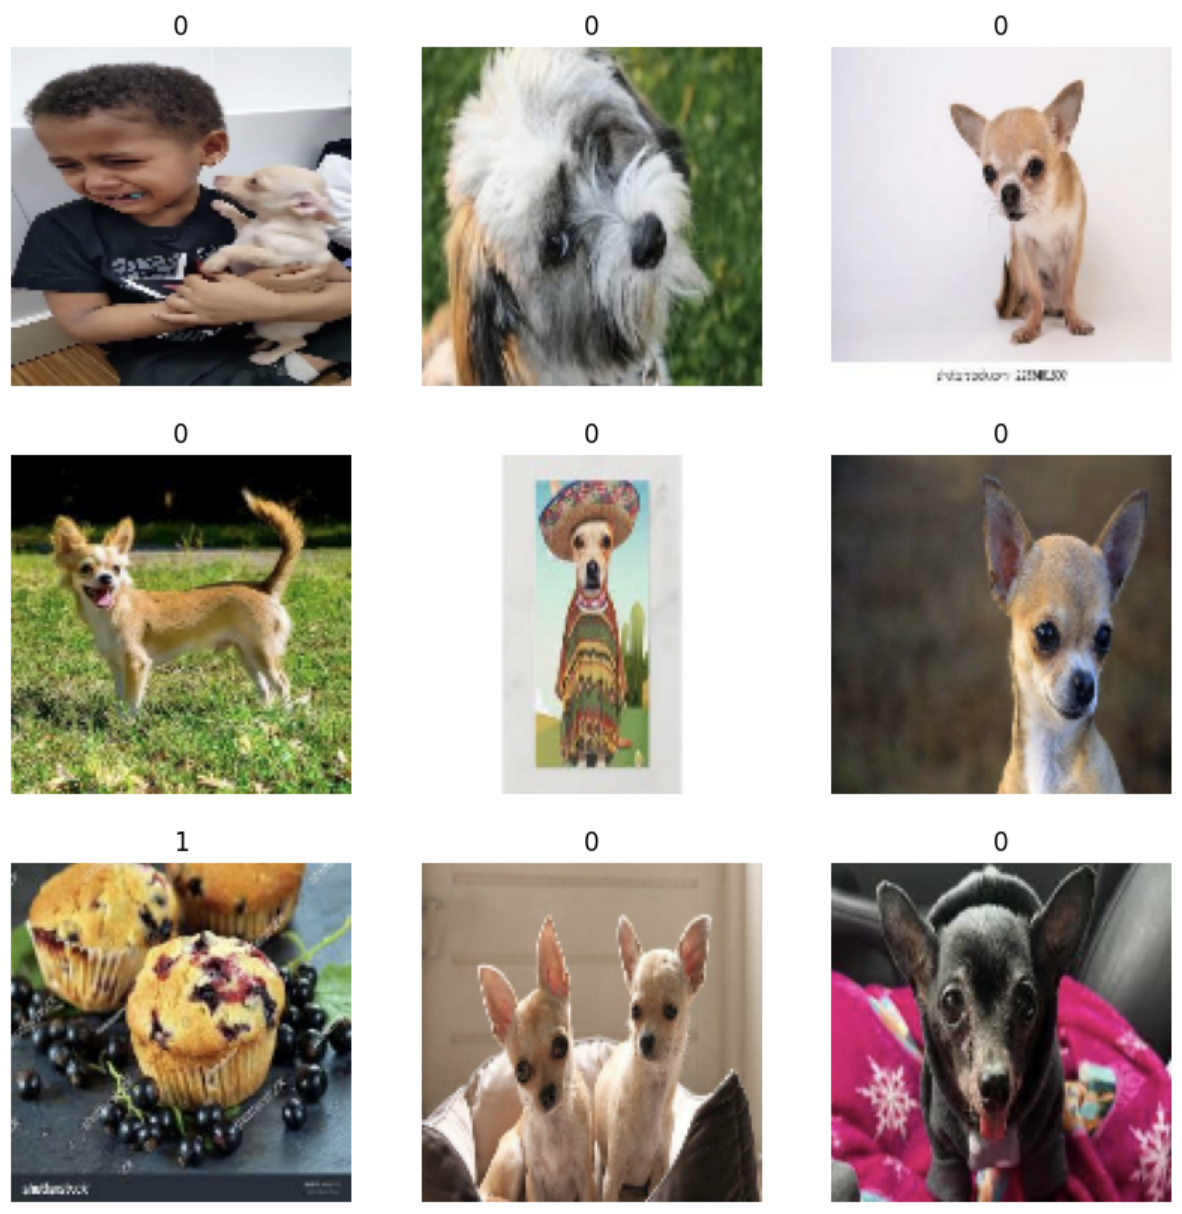
\includegraphics[scale=0.5]{../Images/sampleimages.png}
\end{figure}
As you can see muffin label is 0 and chihuahua label is 1.
\section{Preprocessing}
Certainly when dealing with data it is good to always make some improvement such as cleaning the data so that you have better results. In fact, the dataset was delivered without having duplicate images, which already represents a first step of preprocessing. In addition, I applied the \textbf{Data augmentation} \cite{dataaug} that is a technique in machine learning used to reduce overfitting when training a machine learning model, by training models on several slightly-modified copies of existing data.
With the help of Keras, it is possible to achieve date augmentation in the following way:
\begin{lstlisting}[language=Python]
data_augmentation = keras.Sequential(
    [
        layers.RandomFlip("horizontal"),
        layers.RandomRotation(0.1),
    ]
)
\end{lstlisting}
Here is graphically what the transformation looks like:
\begin{figure}[hbtp]
\caption{Data augmentation applied in a specific image}
\centering
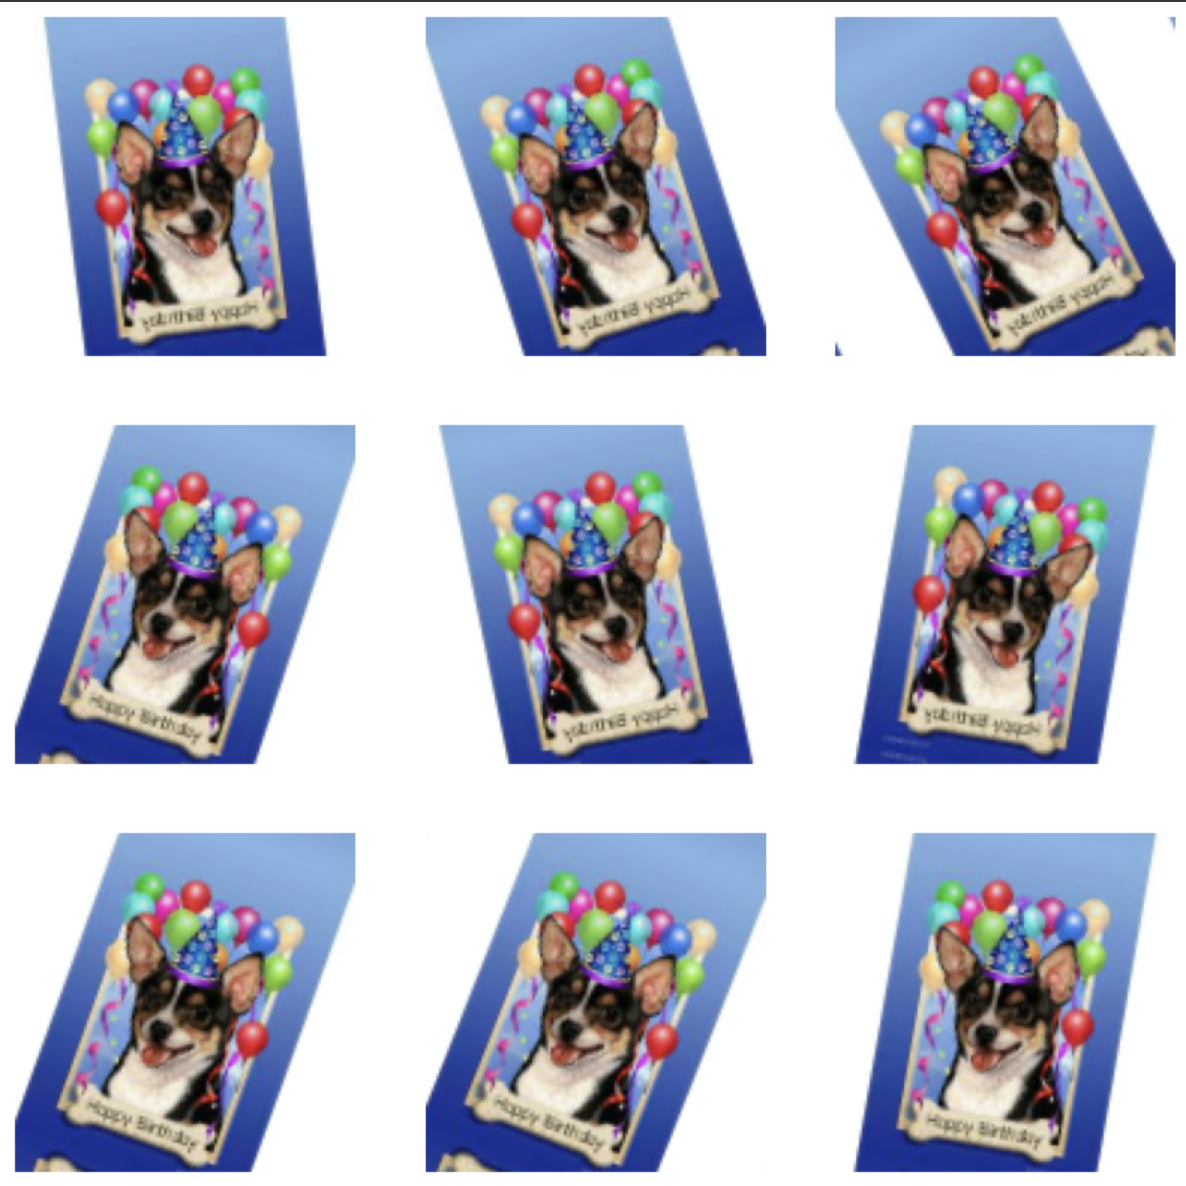
\includegraphics[scale=0.5]{../Images/dataaug.png}
\end{figure}
In order to complete the preprocessing I applied the data augmentation transformation to the input and I performed normalization of pixel values in the range [0, 255] to values in the range [0, 1], indeed this helps stabilize the training of the model. To conclude, this line 
\texttt{train\_images = train\_images.prefetch(tf.data.AUTOTUNE)} optimizes the data loading process during model training, allowing the model to work more efficiently and reducing the waiting time between data batches.


\chapter{Neural Network Models} \label{ch:nnm}
In this chapter we are going to examine the models that have been made in order to solve the binary classification task.
All models were trained using the principle of K-Fold cross validation. In this case the \texttt{K = 5}. For the results of the experiments please refer to the Chapter \ref{ch:experiments} while for the discussion of the experiments please refer to the Chapter \ref{ch:discussion}.

\section{K-fold cross validation (K = 5)}
Cross-validation is a statistical method used to estimate the skill of machine learning models.The procedure has a single parameter called k that refers to the number of groups that a given data sample is to be split into. As such, the procedure is often called k-fold cross-validation. When a specific value for k is chosen, it may be used in place of k in the reference to the model such as k=5 becoming 5-fold cross-validation, the one used in this project. \cite{kfold}.
The general rules are the following:
\begin{enumerate}
\item Shuffle the dataset randomly
\item Split the dataset into k groups
\item For each group:
\begin{itemize}
\item Take the group as a hold out or test data set
\item Take the remaining groups as a training data set
\item Fit a model on the training set and evaluate it on the test set
\item Retain the evaluation score and discard the model
\end{itemize}
\item Summarize the skill of the model using the sample of model evaluation scores
\end{enumerate}
Let's take a look at its mathematical formalization.
Let $S$ be our entire dataset \cite{kfoldmath}. We partition $S$ in $K$ subsets (also known as folds) $S_1, \ldots, S_K$ of size $m / K$ each (assume for simplicity that $K$ divides $m$).The $K$-fold $C V$ estimate of $\mathbb{E}\left[\ell_{\mathcal{D}}(A)\right]$ on $S$, denoted by $\ell_S^{\mathrm{cv}}(A)$, is then computed as follows: we run $A$ on each training part $S_{-i}$ of the folds $i=1, \ldots, K$ and obtain the predictors $h_1=$ $A\left(S_{-i}\right), \ldots, h_K=A\left(S_{-K}\right)$. We then compute the (rescaled) errors on the testing part of each fold,
$$
\ell_{S_i}\left(h_i\right)=\frac{K}{m} \sum_{(\boldsymbol{x}, y) \in S_i} \ell\left(y, h_i(\boldsymbol{x})\right)
$$
Finally, we compute the CV estimate by averaging these errors
$$
\ell_S^{\mathrm{cv}}(A)=\frac{1}{K} \sum_{i=1}^K \ell_{S_i}\left(h_i\right)
$$
\section{Multi-Layer Perceptron (MLP)}
A multilayer perceptron (MLP) is a feedforward artificial neural network, consisting of fully connected neurons with a nonlinear kind of activation function, organized in at least three layers, notable for being able to distinguish data that is not linearly separable. \cite{mlp}
During the project, I developed 3 different MLP models so that I could conduct different experiments and understand the performance of them.
\subsection{First MLP Model}
Here are the MLP architecture:
\begin{itemize}
\item \texttt{inputs = tf.keras.Input(shape=input\_shape)}: model's input with the input\_shape size. In this case (128, 128, 3)
\item \texttt{x = layers.Flatten()(inputs)}: Converts 2D input (an image) to a 1D vector
\item \texttt{x = layers.Dense(256, activation='relu')(x)}: Fully connected layer (dense) with 256 neurons and ReLU activation
\item \texttt{x = layers.Dropout(0.5)(x)}: This dropout layer introduces regularization into the network. The parameter 0.5 indicates that 50\% of the neurons exiting this layer are randomly switched off during training.
\item \texttt{x = layers.Dense(128, activation='relu')(x)}: Other fully connected layer with 128 neurons and ReLU activation.
\item \texttt{x = layers.Dropout(0.5)(x)}: Another dropout layer for further regularization.
\item \texttt{activation = 'sigmoid'}: Here the activation function for the last layer is specified. In your case, you are using 'sigmoid,' which is commonly used in binary classification problems where the output must be a probability between 0 and 1 for each class.
\item \texttt{outputs = layers.Dense(num\_classes, activation=activation)(x)}. \\
num\_classes = 1. This is the last layer of the model, which returns the output.
Then these are the technical details of the setup:
\begin{itemize}
\item \texttt{batch\_size =  32}. Indicates how many data examples are processed together before updating the weights.
\item \texttt{optimizer='adam'}. The optimizer is the algorithm that adjusts the model weights during training to minimize the cost function. It is a stochastic gradient descent method.
\item \texttt{loss = 'binary\_crossentropy'}. It specifies the cost function (or loss function) that will be used to evaluate how well the model is fitting the data during training. This cross-entropy loss is user for binary (0 or 1) classification applications.
\item \texttt{metrics=[zero\_one\_loss\_func]}: this param specifies the evaluation metrics that will be calculated during model training. In this case I used a custom function called \texttt{zero\_one\_loss\_func}. It requires two parameters: \texttt{y\_true} , the real associated label and the \texttt{y\_pred}, the ones predicted by the model. Then:
\begin{itemize}
\item Transforms predicted probabilities into binary labels (0 or 1)
\item Compare the predicted binary labels with the actual labels
\item Calculate the zero-one loss as the average of the errors.
\end{itemize}
\end{itemize}
\end{itemize}
\subsection{Hypertuning parameter for MLP}
Hyper-parameters are parameters that are not directly learnt within estimators.
In order to obtain better results I decided to do an hypertuning of the params using the \textbf{GridSearchCV} from the library \texttt{sklearn.model\_selection}.  GridSearchCV exhaustively considers all parameter combinations from a paramater grid \cite{scikitgs}.
Due the amount of the time spent for the exhaustive combination I choose just two different learning rate \texttt{0.001} and  \texttt{0.01}.
After wrapping the mlp keras into a KerasClassifier I can integrate the scikit-learn flow and run GridSearch. Here the results:
\begin{lstlisting}
Highest score is 0.5403 with {'learning_rate': 0.001, 'optimizer': <class 'keras.optimizers.adam.Adam'>} 

List in descending order:
0.5403 --> {'learning_rate': 0.001, 'optimizer': <class 'keras.optimizers.adam.Adam'>} 
0.5119 --> {'learning_rate': 0.01, 'optimizer': <class 'keras.optimizers.adam.Adam'>} 
\end{lstlisting}
So in this case with a learning rate of \texttt{0.001} the accuracy is better.
\subsection{First MLP Model after Hypertuning}
I trained the same mlp but with different learning rate as discussed above.
The results are quite similar as you can see from the Table \ref{table:mlp1hyp} so I spent some times to create other two mlp architecture.
\subsection{Second MLP Model}
In the second MLP Model I added two fully connected layer(dense) after the 0.5 Dropout of the first MLP Model.
\begin{center}
\begin{tabular}{|l|l|l|}
\hline
\textbf{Layer (type)} & \textbf{Output Shape} & \textbf{Param \#} \\
\hline
input\_7 (InputLayer) & [(None, 128, 128, 3)] & 0 \\
\hline
flatten\_5 (Flatten) & (None, 49152) & 0 \\
\hline
dense\_15 (Dense) & (None, 256) & 12,583,168 \\
\hline
dropout\_10 (Dropout) & (None, 256) & 0 \\
\hline
dense\_16 (Dense) & (None, 128) & 32,896 \\
\hline
dropout\_11 (Dropout) & (None, 128) & 0 \\
\hline
dense\_17 (Dense) & (None, 64) & 8,256 \\
\hline
dropout\_12 (Dropout) & (None, 64) & 0 \\
\hline
dense\_18 (Dense) & (None, 32) & 2,080 \\
\hline
dropout\_13 (Dropout) & (None, 32) & 0 \\
\hline
dense\_19 (Dense) & (None, 1) & 33 \\
\hline
\multicolumn{3}{|c|}{Total params: 12,626,433} \\
\hline
\multicolumn{3}{|c|}{Trainable params: 12,626,433} \\
\hline
\multicolumn{3}{|c|}{Non-trainable params: 0} \\
\hline
\end{tabular}
\end{center}
Also in this case, the performance are not so high as reported in the Table. I executed a 10 epoch training and here the results:
\begin{center}
\begin{tabular}{|c|c|c|}
\hline
\textbf{Epoch} & \textbf{Loss} & \textbf{Accuracy} \\
\hline
1/10 & 1083.8823 & 0.4843 \\
\hline
2/10 & 10.3901 & 0.5398 \\
\hline
3/10 & 9.8943 & 0.5405 \\
\hline
4/10 & 9.4855 & 0.5398 \\
\hline
5/10 & 9.1378 & 0.5400 \\
\hline
6/10 & 8.7128 & 0.5405 \\
\hline
7/10 & 8.3303 & 0.5407 \\
\hline
8/10 & 7.9671 & 0.5407 \\
\hline
9/10 & 7.6214 & 0.5407 \\
\hline
\end{tabular}
\end{center}
\subsection{Third MLP Model}
The third MLP Model has 3 fully connected layers (512,256,128) with a Dropout for each layer of 0.3. Here the results:
\begin{center}
\begin{tabular}{|c|c|c|}
\hline
Epoch & Loss & Accuracy \\
\hline
1 & 900.3068 & 0.5039 \\
\hline
2 & 27.8657 & 0.5172 \\
\hline
3 & 16.0389 & 0.5398 \\
\hline
4 & 14.6262 & 0.5394 \\
\hline
5 & 13.1948 & 0.5400 \\
\hline
6 & 12.0603 & 0.5407 \\
\hline
7 & 11.3178 & 0.5405 \\
\hline
8 & 10.7011 & 0.5394 \\
\hline
9 & 9.8406 & 0.5400 \\
\hline
10 & 9.1993 & 0.5400 \\
\hline
\end{tabular}
\end{center}
\section{Convolutional Neural Network (CNN)}
A \textbf{Convolutional Neural Network}, also known as CNN or ConvNet, is a class of neural networks that specializes in processing data that has a grid-like topology, such as an image. A digital image is a binary representation of visual data. It contains a series of pixels arranged in a grid-like fashion that contains pixel values to denote how bright and what color each pixel should be. \cite{cnn}
\begin{figure}[hbtp]
\caption{Example of CNN architecture}
\centering
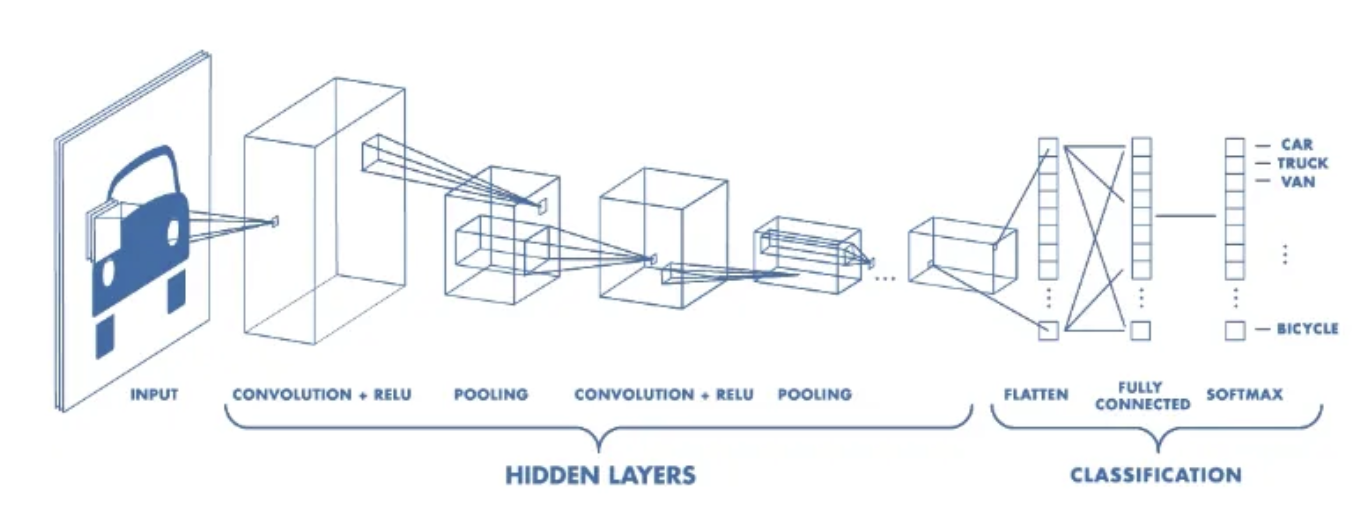
\includegraphics[scale=0.5]{../Images/cnnarch.png}
\end{figure}
\subsection{CNN Model}
During the project, I trained a CNN model to solve the binary classification problem. Here are the details of the architecture:
\begin{itemize}
\item \texttt{inputs = tf.keras.Input(shape=input\_shape)}. Define a input layer for the model. 
\item \texttt{x = layers.Rescaling(1.0 / 255)(inputs)}. Rescaling for pixel normalization.
\item \texttt{x = layers.Conv2D(128, 3, strides=2, padding="same", activation="relu")(x)}. This is a 2D convolution layer with 128 filters, a kernel size of 3x3, a stride of 2 (i.e., displacement of 2 pixels at a time), and a ReLU activation function. This layer extracts features from the image.
\item \texttt{x = layers.MaxPooling2D(3, strides=2, padding="same")(x)}.This is a 2D max-pooling layer with a pool size of 3x3, a stride of 2, and equal "padding." Max-pooling reduces the size of the feature maps extracted from the convolution layer.
\item \texttt{Middle block the same of the previous two step}.
\item \texttt{x = layers.GlobalAveragePooling2D()(x)}.This layer performs "Global Average Pooling" on the resulting feature maps. Global Average Pooling calculates the average of the values in each feature map, producing a compact representation of the features.
\item \texttt{x = layers.Dropout(0.5)(x)}. This is a dropout level that helps prevent overfitting. It randomly deactivates 50\% of the neurons during training.
\item \texttt{activation = "sigmoid"}.The activation function for the output layer is defined as "sigmoid," which is commonly used for binary classification problems.
\item \texttt{outputs = layers.Dense(num\_classes, activation=activation)(x)}.this is the output layer that produces the final predictions of the model. The number of neurons corresponds to the number of classes specified by the num\_classes parameter, and the activation function is "sigmoid" for the binary classification problem.
\end{itemize}
Then these are the technical details of the setup:
\begin{itemize}
\item \texttt{batch\_size =  32}. Indicates how many data examples are processed together before updating the weights.
\item \texttt{optimizer=keras.optimizers.Adam(1e-3)}. The optimizer is the algorithm that adjusts the model weights during training to minimize the cost function. It is a stochastic gradient descent method. I specified the learning rate to \texttt{0.001}
\item \texttt{loss = 'binary\_crossentropy'}. It specifies the cost function (or loss function) that will be used to evaluate how well the model is fitting the data during training. This cross-entropy loss is user for binary (0 or 1) classification applications.
\item \texttt{metrics=[zero\_one\_loss\_func]}: this param specifies the evaluation metrics that will be calculated during model training. In this case I used a custom function called \texttt{zero\_one\_loss\_func}. It requires two parameters: \texttt{y\_true} , the real associated label and the \texttt{y\_pred}, the ones predicted by the model. Then:
\begin{itemize}
\item Transforms predicted probabilities into binary labels (0 or 1)
\item Compare the predicted binary labels with the actual labels
\item Calculate the zero-one loss as the average of the errors.
\end{itemize}
\end{itemize}
The result of the experiments is reported in the Table \ref{table:cnn}.
\section{Deep Residual learning (ResNet50)}
ResNet-50 is a convolutional neural network that is 50 layers deep. You can load a pretrained version of the neural network trained on more than a million images from the ImageNet database \cite{imagenet}.The pretrained neural network can classify images into 1000 object categories, such as keyboard, mouse, pencil, and many animals. As a result, the neural network has learned rich feature representations for a wide range of images.The main innovation in ResNet is the introduction of \textbf{residual blocks}. In a residual block, the input is added to the output, allowing the model to learn the differences between the two rather than trying to learn the entire mapping. This makes training much more stable for very deep networks.ResNet-50 is often used for \textbf{transfer learning}.As a result, the model weights have already learned high-level representations that can be used for various computer vision tasks.
\begin{figure}[hbtp]
\caption{ResNet50 Architecture}
\centering
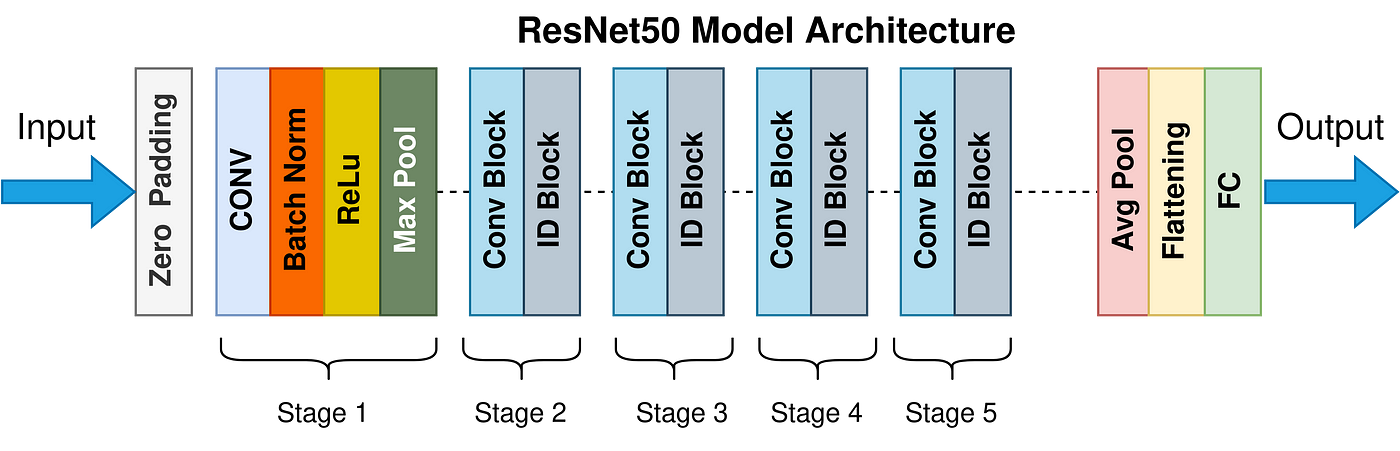
\includegraphics[scale=0.3]{../Images/resnet50arch.png}
\end{figure}
\subsection{ResNet50 Model}
Here are the details of the architecture:
\begin{itemize}
\item \texttt{base\_model = ResNet50(} \\
    \texttt{weights='imagenet',} \\
    \texttt{include\_top=False,} \\
    \texttt{input\_tensor=Input(shape=input\_shape))}. Loads the ResNet50 pre-trained model.\\ 
 	\texttt{weights='imagenet'} indicates that we want to use the pre-trained weights provided by ImageNet.\\
  \texttt{include\_top=False} means that we do not want to include the fully connected layers (top layers) of the model, and \\
   \texttt{input\_tensor=Input(shape=input\_shape)} specifies the shape of the input tensor.
\item \texttt{x = base\_model.output}\\
\texttt{x = GlobalAveragePooling2D()(x)} \\
\texttt{x = Dense(256, activation='relu')(x)} \\
\texttt{predictions = Dense(num\_classes, activation='sigmoid')(x)}. It adds a Global Average Pooling layer and a fully connected layer. Here, the output of the ResNet50 model is passed through a 2D Global Average Pooling layer, which averages the spatial features for each channel. Then, a second fully connected layer with 256 units and ReLU activation is added, followed by an output layer with a number of units equal to num\_classes and sigmoid activation. The latter layer will return the probabilities associated with each class.
\item \texttt{model = Model(inputs=base\_model.input, outputs=predictions)}.Using the Model object, model inputs (the same inputs as the ResNet50 model) and outputs (the predictions tensor created in the previous step) are specified to create the final model.
\item \texttt{for layer in base\_model.layers: layer.trainable = False}.In this for loop, all layers of the basic ResNet50 model are iterated and their weights are set as non-trainable (they will not be updated during training of the new model). This is useful when using pre-trained weights for feature extraction and you want to prevent them from being overwritten during training.
\end{itemize}
Then these are the technical details of the setup:
\begin{itemize}
\item \texttt{batch\_size =  32}. Indicates how many data examples are processed together before updating the weights.
\item \texttt{optimizer=keras.optimizers.Adam(1e-3)}. The optimizer is the algorithm that adjusts the model weights during training to minimize the cost function. It is a stochastic gradient descent method. I specified the learning rate to \texttt{0.001}
\item \texttt{loss = 'binary\_crossentropy'}. It specifies the cost function (or loss function) that will be used to evaluate how well the model is fitting the data during training. This cross-entropy loss is user for binary (0 or 1) classification applications.
\item \texttt{metrics=['accuracy']}: this param specifies the evaluation metrics that will be calculated during model training. In this case I have the accuracy metric.
\end{itemize}


%
%			BIBLIOGRAFIA
%

\bibliographystyle{unsrt}
\bibliography{bibliografia}
\addcontentsline{toc}{chapter}{References}


\end{document}


 
